\documentclass[12pt,letterpaper,titlepage,oneside]{article}
\usepackage[utf8]{inputenc}
\usepackage{amsmath}
\usepackage{amsfonts}
\usepackage{amssymb}
\usepackage{seqsplit}
\usepackage{graphicx}
\title{Using Data Analytics to Garner an Understanding of Brilliance in Hollywood: One Out of 100 Actors at the Academy Awards is a Genius}
\author{
	Zachary Bricker  \\
	zbricker@my.harrisburgu.edu
	\and
	Douglas Bahr Rumbaugh \\
	dbrumbaugh@my.harrisburgu.edu
	\and 
	Chad Van Chu \\
	cvchu@my.harrisburgu.edu
	\\
	\\
	Harrisburg University of Science and Technology
}

\date{}

\begin{document}
\maketitle
\section*{Abstract}
\tableofcontents
\pagebreak


\section{Introduction}
In recent years, it has become fashionable to possess a high IQ. It is, then, no big surprise that recent years have also seen a massive surge in public figures reported IQ scores. Of particular interest to the authors are the claims of those in the entertainment industry.

One needs not look terribly hard in order to stumble across news articles, both in traditional media and the tabloid press, claiming to posses a list of the smartest celebrities. Interestingly enough, in the authors' experience, such articles rarely provide evidence for their claims.

As such, the authors determined that it would be an interesting exercise to examine the implications of the truth of these reported IQ scores. There are 3,000 seats at the Academy Awards--so what is the probability of random chance alone bringing such an assortment of geniuses into the same room? That is the question this study hopes to answer.
\section{Review of Literature}

\section{Methods}

\subsection{Data Collection}
\label{methoddata}
In order to obtain the data for this analysis, reported IQ scores for celebrities were aggregated from several Internet sources. Unsurprisingly, for several celebrities, there were discrepancies between IQs reported from source to source. These discrepancies are discussed in further detail in the Discussion section. For the primary analysis though, a single IQ value per person was required. In these cases, the most frequently occurring reported IQ was selected, under the assumption that the most frequently repeated score was the one with the most popular acceptance.


\subsection{Basic Probability Analysis}
\label{probanal}
Using the IQ distribution, each individual was assigned the probability of having their reported IQ score. Then, the probability of all of these individuals being in the same sample, given their IQ scores, was calculated using the following formula:

\begin{equation}
3000 * \prod_{k=1}^n p(i_k)
\end{equation}
Where $i_k$ is the IQ score of the $k$th celebrity and $p(i)$ is the probability function, returning the proportion of people with the IQ score $i$, and there were $n$ celebrities sampled.

The number 3,000 represents the 3,000 seats at the Academy Awards. In truth, there are not a full 3,000 opportunities, because there are $n$ celebrities sampled--so in the 3,000 seats of the Academy Awards, there are only $\frac{3000}{n}$ chances for all $n$ celebrities to be in the 3,000 seats. However, in the interest of giving the celebrities a fighting chance, the probability is calculated in terms of 3000 opportunities, not $\frac{3000}{n}$ opportunities.

\subsection{Monte Carlo Simulation} 

\section{Results}
\subsection{IQ Scores}

\begin{figure}[h!]
\caption{Histogram for Reported IQ Distribution}
\label{iqhist}
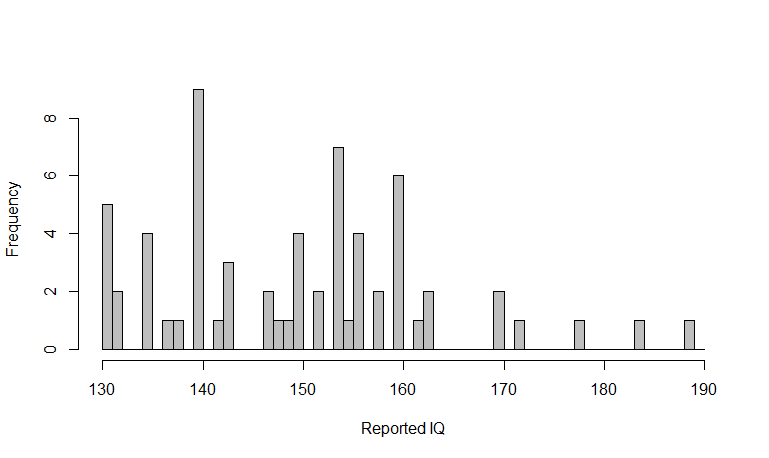
\includegraphics[scale=.5]{reported-iq}
\end{figure}

\subsection{Probability Analysis}
Using the technique defined in Section \ref{probanal}, the probability of all of the sampled IQ scores being in the same random sample of 3,000 individuals is $3.4463 * 10^{-225}$.

\subsection{Monte Carlo Simulation}
\begin{figure}[h!]
\caption{Histogram for Expected IQ Distribution}
\label{iqhist}
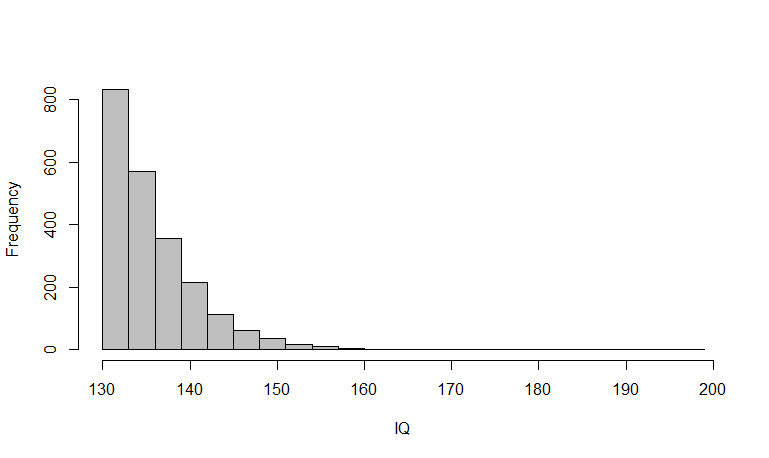
\includegraphics[scale=.5]{expected-above-average}
\end{figure}

\section{Discussion}
The result of $3.4463 * 10^{-225}$ being the probability of all the sampled IQ scores being in the same random sample of 3,000 individuals is striking--and the number is far worse than the authors had initially suspected. To put it in perspective, this probability in terms of odds is 1 chance in \seqsplit{3446300000000000000
0000000000000000000
0000000000000000000
0000000000000000000
0000000000000000000
0000000000000000000
0000000000000000000
0000000000000000000
0000000000000000000
0000000000000000000
0000000000000000000
00000000000000000}. To be fair, a sample of the top reported IQ scores from the top entertainers is not exactly random, however this probability is still ridiculously small.

In addition, another interesting observation is the preponderance of zero-terminated IQ scores. Among the top four most frequent IQ scores are 130, 140, and 160. The IQ score of 140 alone constitutes almost 14\% of the 65 IQ scores collected. Almost 37\% of all collected scores end in a 0, but only 8\% are 130. This is not the behavior that would be expected from the IQ distribution at 130 and above, where the majority of scores are 130 as shown in Figure \ref{iqhist}. In fact, the distribution of scores obtained from the literature looks nothing like the expected.

It is possible that the prevalence of these zero-terminated IQ scores is due to rounding on the part of those making the IQ score reports. It is notable that, for certain individuals, some sources cited exact scores, and others admitted to approximation with language along the lines of "x's IQ score has been reported to be around 140". This is an interesting phenomena, considering that an IQ score is typically something that is either known, or not known--there isn't much room for approximation.

It is possible that this approximation is indicative of the inventive spirit of journalism. Or, perhaps it merely facilitates the rounding up of IQ scores. It seems unlikely that the field of entertainment specifically attracts individuals with exact zero-terminated IQ scores more than it does individuals with non-zero-terminated scores.

It is also perhaps notable that many individuals had several reported scores. As discussed in Section \ref{methoddata}, for the probability analysis only the most frequently reported score was used, however 26\% of the individuals in the sample had at least two different IQ scores referenced in the literature. Occasionally, these reported scores differed by as many as 25 IQ points. This is five points less than two standard deviations from the mean on the IQ distribution. That is quite the difference!

\end{document}